%%%%%%%%%%%%%%%%%%%%%%%%%%%%%%%%%%%%%%%%%%%%%%%%%%%%%%%%%%%%%%%%
\section{Master Algorithms}
\label{sec:impl_algorithms}

This section addresses SR-11-03 (numerical treatment of algebraic loops) and explains how \syssimx{} realizes the master algorithms introduced in Section~\ref{sec:234_cosim_execution_strategies}.
The structural analysis of Section~\ref{sec:impl_structural} already provides the execution generations and the detected algebraic loops.
Section~\ref{sec:impl_algebraic_loops} already defined the SCC-local loop solver.
The present section therefore focuses on the orchestration of one macro step by the concrete classes \texttt{JacobiAlgorithm}, \texttt{GaussSeidelAlgorithm}, and \texttt{IJCSAAlgorithm}.
Hybrid event handling is excluded here and is explained in Section~\ref{sec:impl_hybrid}.

%%%%%%%%%%%%%%%%%%%%%%%%%%%%%%%%%%%%%%
\subsection{Scope and Shared Metadata}
\label{sec:impl_algorithms_scope}

All master algorithms consume the same execution metadata stored on the \texttt{System} instance during initialization.
The list \pyfn{execution\_order} defines the generation order, \pyfn{algebraic\_loops} identifies the loop blocks, and \pyfn{\_set\_inputs\_for\_generation()} propagates signal values to the destination input ports of one generation.
The Jacobi and Gauss--Seidel algorithms reuse the SCC-local solver of Section~\ref{sec:impl_algebraic_loops}.
The global \pyfn{IJCSAAlgorithm} replaces this local treatment by one global interface solve before the macro steps are executed.

Across all three algorithms, one macro step consists of two tasks.
First, the interface values at the current communication point are propagated and, if required, corrected so that the zero-delay couplings are consistent.
Second, the components advance from $t$ to $t+\Delta t$ by calling \texttt{do\_step(t, dt)}.
The algorithms differ only in how these tasks are ordered across the generations and in whether the interface correction is carried out locally per loop block or globally for the complete system.

Figure~\ref{fig:impl_algorithms_jacobi_gs} summarizes the implementation-level execution flow of the two explicit continuous master algorithms.

\begin{figure}[!htbp]
    \vspace{-1em}
    \centering
    \begin{subfigure}[t]{0.48\linewidth}
        \centering
        \begin{minipage}[t][9.8cm][t]{\linewidth}
            \vspace{0pt}
            \centering
            \includegraphics[width=\linewidth]{diagrams/out/pdf/execution/Jacobi_Algorithm.pdf}
        \end{minipage}
        \caption{Jacobi execution. All generations are prepared first. The component steps are executed only afterwards.}
        \label{fig:impl_algorithms_jacobi}
    \end{subfigure}
    \hfill
    \begin{subfigure}[t]{0.48\linewidth}
        \centering
        \begin{minipage}[t][9.8cm][t]{\linewidth}
            \vspace{0pt}
            \centering
            \includegraphics[width=\linewidth]{diagrams/out/pdf/execution/Gauss_Seidel_Algorithm.pdf}
        \end{minipage}
        \caption{Gauss--Seidel execution. Each generation is prepared and stepped immediately before the next one is processed.}
        \label{fig:impl_algorithms_gs}
    \end{subfigure}
    \caption{Implementation-level execution diagrams of the explicit continuous master algorithms.}
    \label{fig:impl_algorithms_jacobi_gs}
    \vspace{-1em}
\end{figure}

%%%%%%%%%%%%%%%%%%%%%%%%%%%%%%%%%%%%%%
\subsection{Jacobi Algorithm}
\label{sec:impl_algorithms_jacobi}

The class \texttt{JacobiAlgorithm} realizes the explicit non-iterative scheme of Section~\ref{sec:234_cosim_execution_strategies} by structuring one macro step in two phases over \texttt{execution\_order}.
In the first phase, the algorithm iterates through the generations.
For each one, it calls \pyfn{\_set\_inputs\_for\_generation(gen, t)} to stage the interface values at the current communication point.
If the generation contains algebraic loops, it then invokes \pyfn{solve\_algebraic\_scc\_ijcsa(system, loop, t)}.
In the second phase, the algorithm iterates through the generations a second time.
Every component of each generation is advanced by one step through \texttt{do\_step(t, dt)} with the interface values frozen at $t$.
Because no component advances before all interface values have been staged, components in later generations still read the output values produced at the previous communication point.
This is how the Jacobi property works at the implementation level.
All simulation units use the same communication-point snapshot.
The current implementation preserves this semantics through a serial loop over the generations, so the second phase would admit parallel execution of the component steps, but \syssimx{} does not yet exploit this.

%%%%%%%%%%%%%%%%%%%%%%%%%%%%%%%%%%%%%%

\subsection{Gauss--Seidel Algorithm}
\label{sec:impl_algorithms_gs}

The class \texttt{GaussSeidelAlgorithm} collapses the two phases of the Jacobi implementation into a single pass over \texttt{execution\_order}.
For each generation, the algorithm first stages the interface values through \pyfn{\_set\_inputs\_for\_generation(gen, t)}.
It then solves every loop block contained in that generation through \pyfn{solve\_algebraic\_scc\_ijcsa(system, loop, t)}.
The execution of \texttt{do\_step(t, dt)} moves every component of the generation to $t+\Delta t$.
The output ports of the components in earlier generations therefore already hold the values at $t+\Delta t$ when the inputs of a later generation are staged.
A call of \pyfn{\_set\_inputs\_for\_generation()} on the next generation propagates these fresh values into the destination ports.
This within-step visibility of updated outputs is the only algorithmic difference to the Jacobi implementation.
The local SCC solver, the input-staging routine, and the structural metadata on \texttt{System} are reused unchanged, which is why the two classes share the orchestration skeleton of Section~\ref{sec:impl_algorithms_scope} and differ only in where the \texttt{do\_step(t, dt)} call is placed relative to the generation loop.
The sequential per-generation ordering also implies that the Gauss--Seidel algorithm does not exploit the parallelism that the Jacobi second phase would admit in principle.

%%%%%%%%%%%%%%%%%%%%%%%%%%%%%%%%%%%%%%
%%%%%%%%%%%%%%%%%%%%%%%%%%%%%%%%%%%%%%
\subsection{Global IJCSA Algorithm}
\label{sec:impl_algorithms_ijcsa}

The class \texttt{IJCSAAlgorithm} provides a global counterpart to the SCC-local solver of Section~\ref{sec:impl_algebraic_loops}.
It implements the original Sicklinger formulation~\cite{sicklinger_interface_2014}, which treats the full set of zero-delay interface unknowns of the scenario as one coupled Newton system.

Its \texttt{step()} method runs in two phases.
The first phase calls \pyfn{solve\_global\_interface\_ijcsa(system, t)}.
This routine uses \pyfn{collect\_global\_interface\_unknowns()} to build the global unknown vector and the driver map.
A Newton iteration is then applied to the residual $\mathcal{R}(U)=U-\widehat{U}(U)$ with frozen component states, as in the local solver.
A damped-gradient fallback stabilizes the update when the Jacobian is singular.
After convergence, the solved interface values are written to the destination input ports.
In the second phase, \texttt{step()} traverses \texttt{execution\_order} and calls \texttt{do\_step(t, dt)} on every component.

Several elements of the original Sicklinger formulation are deliberately omitted in \syssimx{}.
The constraint operator is restricted to the signal-assignment form $U=\widehat{U}(U)$.
A general nonlinear interface constraint $L(U,Y)=0$ is not supported.
The inner evaluation reuses the side-effect-free \pyfn{evaluate\_outputs(inputs)} contract and keeps component states frozen at $t$.
Trial macro steps with rollback are therefore not required.
The interface Jacobian is always assembled by finite differences.
Directional derivatives exposed by the simulation units are not requested even when available.
Input extrapolation between communication points and an explicit relaxation factor are also absent.
The fixed point is reached with unit step length or with the damped-gradient fallback.

The global solve is mathematically redundant when the zero-delay SCCs are disjoint.
In that case its block-diagonal Jacobian is equivalent to running the local solver of Section~\ref{sec:impl_algebraic_loops} once per SCC, and the two variants produce the same fixed point in the same number of Newton iterations.
\texttt{IJCSAAlgorithm} is therefore included mainly for completeness and as a reference implementation of the original Sicklinger scheme.
The default orchestration path is \texttt{JacobiAlgorithm} or \texttt{GaussSeidelAlgorithm}, which invoke the local solver on demand and avoid assembling one large interface system for every macro step.

%%%%%%%%%%%%%%%%%%%%%%%%%%%%%%%%%%%%%%
\subsection{Verification}
\label{sec:impl_algorithms_verification}

Verification of the three master algorithms uses a small feedback scenario which combines a constant source, a gain block, a subtractor, and an integrator.
The only delayed edge is the one entering the integrator, so the zero-delay graph is acyclic and the structural analysis produces three generations without any SCC.
Figure~\ref{fig:impl_algorithms_verification_system} shows the resulting topology.

\begin{figure}[!htbp]
    \centering
    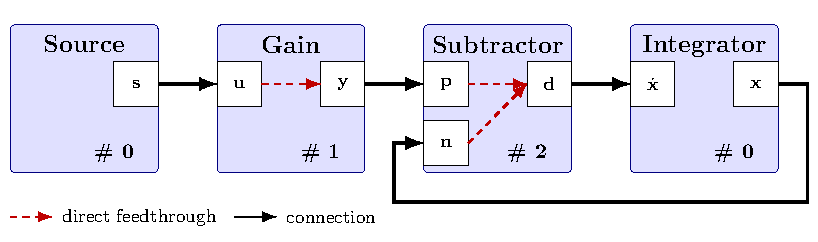
\includegraphics[width=0.85\linewidth]{figures/5_implementation/master_algorithms/master_algorithm_verification.pdf}
    \caption{Topology of the verification scenario. Solid black arrows are port-to-port connections. Dashed red arrows are internal direct-feedthrough relations. The generation index is shown in the lower-right corner of each component. Because the Integrator has no direct feedthrough from $\dot{x}$ to $x$, the inbound edge $\texttt{Subtractor.d} \to \texttt{Integrator.}\dot{x}$ is delayed. This is why the Integrator shares generation~$0$ with the Source and the zero-delay graph remains acyclic.}
    \label{fig:impl_algorithms_verification_system}
\end{figure}

The continuous dynamics reduce to the scalar ODE $\dot{y}=k\,r-y$ with $y(0)=0$.
Its analytical solution
\begin{equation}
    y(t) = k\,r\,\bigl(1-e^{-t}\bigr)
\end{equation}
serves as the reference.

Figure~\ref{fig:impl_algorithms_verification} compares all three algorithms against this reference for four macro step sizes with $k=2$ and $r=1$.

\begin{figure}[t]
    \vspace{-1ex}
    \centering
    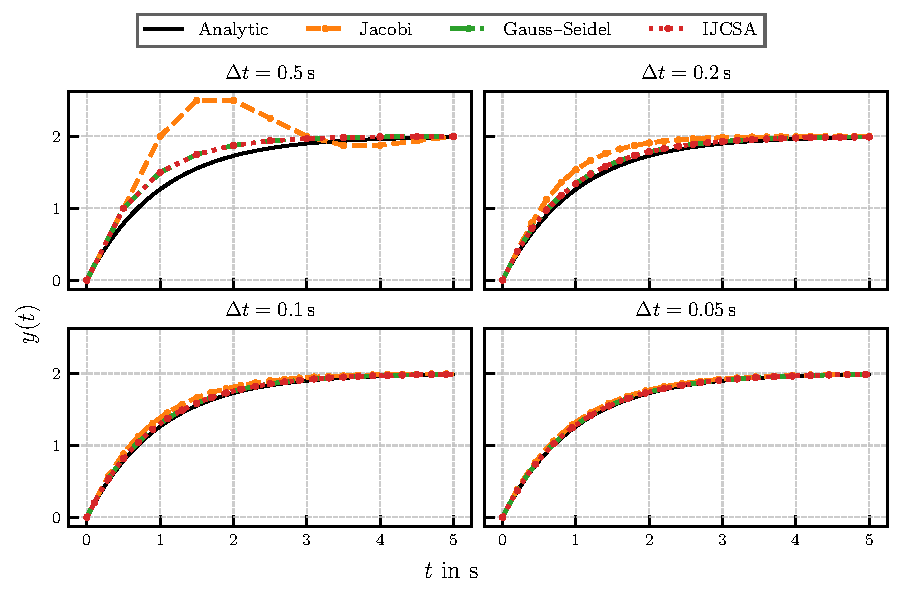
\includegraphics[width=0.9\linewidth]{figures/5_implementation/master_algorithms/algorithm_comparison.pdf}
    \caption{Jacobi, Gauss--Seidel, and Global IJCSA orchestration on a feedback scenario with direct feedthrough and one delayed edge into the integrator. The analytical solution $y(t)=kr(1-e^{-t})$ with $k=2$ and $r=1$ is shown in black. At $\Delta t=0.5\,$s the Jacobi trace overshoots the reference. The Gauss--Seidel and Global IJCSA traces stay close and overlap. All three traces converge to the analytical solution as $\Delta t$ is reduced.}
    \label{fig:impl_algorithms_verification}
\end{figure}

At $\Delta t = 0.5\,$s the Jacobi trace overshoots the analytical solution, while the Gauss--Seidel trace stays close to it.
The overshoot is a direct consequence of the two-phase structure of \texttt{JacobiAlgorithm}.
Components in later generations read output values from the previous communication point, so the feedback through the integrator reaches the subtractor with one macro-step delay.
The Gauss--Seidel pass propagates the updated subtractor output within the same macro step and therefore tracks the reference more closely.
The \texttt{IJCSAAlgorithm} trace overlaps the Gauss--Seidel trace in this scenario.
This is expected because the zero-delay graph is acyclic.
The global solve still contains the zero-delay interface inputs of the Gain and Subtractor components, but it does not resolve an algebraic loop.
After this consistency step, the algorithm advances the generations sequentially.
Its behavior therefore matches the Gauss--Seidel traversal for this example.
All three traces approach the analytical solution as the macro step size is reduced.
This verifies the expected orchestration behavior of the three master algorithms.

The scenario does not exercise algebraic-loop resolution because its zero-delay graph is acyclic.
The SCC-local Newton solve is verified separately in Section~\ref{sec:impl_algebraic_loops}.


